\section{ТЕОРЕТИЧЕСКИЕ СВЕДЕНИЯ}

\subsection{Набор регистров}

В программах на языке ассемблер регистры микропроцессора используются очень интенсивно.
Основные программно-доступные регистры изображены на рисунке~\ref{fig:registers}.

\begin{figure}[htbp]
  \centering
  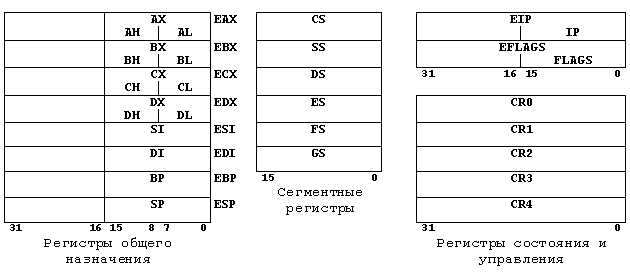
\includegraphics[width=150mm]{pic/registers}
  \caption{Основные регистры 32-разрядных процессоров}\label{fig:registers}
\end{figure}

\textbf{Регистры общего назначения} без каких-либо ограничений могут использоваться
для хранения операндов логических и арифметических операций, компонентов адреса, указателей
на ячейки памяти, однако, каждый из них имеет определенное функциональное назначение:

\begin{itemize}
\item EAX/AX/AH/AL (Accumulator register) --- аккумулятор --- применяется для хранения
  промежуточных данных, а также адресов;
\item EBX/BX/BH/BL (Base register) --- базовый регистр --- применяется для хранения
  промежуточных данных, а также для хранения базового адреса объектов в памяти;
\item ECX/CX/CH/CL (Count register) --- регистр-счетчик --- применяется для хранения
  промежуточных данных, а также в циклических командах, производящих некоторые
  повторяющиеся действия, в качестве счетчика итераций;
\item EDX/DX/DH/DL (Data register) --- регистр данных --- так же, как и регистр EAX/AX/AH/AL, он
  используется для хранения промежуточных данных.
\end{itemize}

\textbf{Сегментные регистры} предназначены для аппаратной поддержки структурной
организации программы в виде отдельных частей, называемых сегментами.
Сегмент представляет собой независимый блок памяти фиксированного размера.
Операционная система размещает сегменты программы в оперативной памяти,
после чего помещает их адреса в соответствующие сегментные регистры.

Микропроцессор поддерживает следующие типы сегментов:

\begin{itemize}
\item сегмент кода --- содержит машинные команды, для доступа к нем у служит регистр CS
  (Code Segment register) --- сегментный регистр кода;
\item сегмент стека --- для доступа к нему служит регистр SS (Stack Segment register) ---
  сегментный регистр стека;
\item сегмент данных --- содержит обрабатываемые программой данные, для доступа к нему
  служит регистр DS (Data Segment register) --- сегментный регистр данных;
\item
  дополнительные сегменты данных --- их адреса должны содержаться в регистрах ES, GS, FS.
\end{itemize}

\subsection{Типы данных}

Микропроцессор аппаратно поддерживает следующие основные типы данных, представленные
на рисунке~\ref{fig:sizes}:

\begin{itemize}
\item байт --- восемь последовательно расположенных битов;
\item слово --- два байта, имеющих последовательные адреса;
\item двойное слово --- четыре байта, расположенные последовательно;
\item учетверенное слово --- восемь байт, расположенные последовательно.
\end{itemize}

\begin{figure}[htbp]
  \centering
  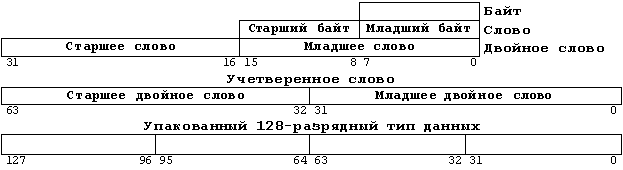
\includegraphics[width=150mm]{pic/sizes}
  \caption{Основные типы данных микропроцессора}\label{fig:sizes}
\end{figure}


\subsection{Структура программы}

Программа на языке ассемблер состоит из строк, содержащих следующие поля:
\textit{метка: команда/директива операнды ;комментарий}.
Все эти поля в отдельных случаях необязательны. 

Текст от символа <<;>> транслятором не анализируется и используется
в качестве комментария.

В машинную команду микропроцессора явно или неявно входят следующие элементы:

\begin{itemize}
\item поле префиксов --- элемент команды, который уточняет либо модифицирует действие этой
  команды;
\item поле кода операции, определяющее действие данной команды;
\item поле операндов --- содержит от нуля до трех элементов.
\end{itemize}

Важной особенностью машинных команд является то, что они не могут манипулировать
одновременно двумя операндами, находящимися в оперативной памяти. По этой причине
возможны только следующие сочетания операндов в команде:
регистр-регистр,
регистр-память,
память-регистр,
регистр-непосредственный операнд,
память-непосредственный операнд.
Из перечисленных сочетаний операндов наиболее часто употребляются регистр - память и
память - регистр.


\subsection{Директивы распределения памяти}

Определение переменных (выделение памяти для переменных в коде программы) в общем
виде записывается следующим образом: \textit{name d* value},
где d* --- одна из псевдокоманд:
\begin{itemize}
\item db --- определить байт;
\item dw --- определить слово (два байта);
\item dd --- определить двойное слово (четыре байта);
\item df или dp --- определить шесть байт (дальний указатель);
\item dq --- определить учетверенное слово (восемь байт);
\item dt --- определить десять байт.
\end{itemize}

\subsection{Режимы адресации}

\textbf{Прямая адресация} --- простейший вид адресации операнда в памяти.

Прямая адресация может быть двух типов:
\begin{itemize}
\item относительная --- используется в командах условного и безусловного перехода;
\item абсолютная --- используется редко.
\end{itemize}

\textbf{Косвенная базовая (регистровая) адресация} --- адрес операнда находится в любом из
регистров общего назначения, кроме SP/ESP и BP/EBP.

Синтаксически в команде этот режим адресации выражается заключением имени регистра в квадратные скобки [].
Например, команда \textit{mov bx, [eax]}
помещает в регистр BX содержимое слова по адресу из сегмента данных со смещением,
хранящимся в регистре EAX, т.е. по адресу DS:EAX.

\textbf{Косвенная базовая (регистровая) адресация со смещением} является дополнением
предыдущей и предназначена для доступа к данным с известным смещением относительно
некоторого базового адреса. Например, команда
\textit{mov bx, [eax + 10h]}
пересылает в регистр BX слово из области памяти по адресу:
содержимое EAX + 10h (DS:EAX+10h).

\textbf{Косвенная индексная адресация со смещением} очень похожа на косвенную базовую
адресацию со смещением, но обладает той особенностью, что позволяет масштабировать
содержимое индексного регистра. Например, в команде
\textit{mov ax, mas[esi*2]}
значение эффективного адреса второго операнда вычисляется выражением MAS + (ESI) * 2.

\textbf{Косвенная базово-индексная адресация} похожа на косвенную базовую адресацию со
смещением. Эффективный адрес формируется как сумма содержимого двух любых регистров
общего назначения: базового и индексного. Например: \textit{mov eax, [esi][edx]}.

\textbf{Косвенная базово-индексная адресация со смещением} вляется дополнением косвенной
базовой индексной адресации. Эффективный адрес формируется как сумма трех составляющих:
содержимого базового регистра, содержимого индексного регистра и значения смещения.
Например, команда \textit{mov eax, [esi + 5][edx]} 
пересылает в регистр EAX двойное слово по адресу: (ESI) + 5 + (EDX).

\textbf{Косвенная базово-индексная адресация со смещением и масштабированием}
объединяет в себе все предыдущие режимы косвенной адресации. Например:
\textit{mov eax, array[ebx][esi*4], ecx}
пересылает в регистр EAX слово из области памяти по адресу array + (ebx) + (esi) * 4.